Důležitou částí této práce je aplikace, která umožňuje pro konkrétní vstupní data vypočítat výnosy fotovoltaické elektrárny a výpočet různých investičních metrik.
Nejdříve je popsána použitá technologie a zdroje dat, následně jsou uvedeny konkrétní příklady výpočtů.

Zdrojový kód aplikace je dostupný na \newline \url{https://github.com/yoptohlejepeta/Optimalizace-FVE/}

\section{Popis aplikace}

Veškerá implementace byla provedena v programovacím jazyce Python. Python je moderní programovací jazyk, který je využívaný v mnoha oblastech, například v analýze dat, strojovém učení nebo vývoji webových aplikací.



\subsection{Použité technologie}

\subsubsection{FastAPI} je moderní webový framework pro tvorbu REST API.
Tvoří základ aplikace.
FastAPI automaticky generuje interkaktivní api dokumentaci, která slouží jako jednoduché uživatelské rozhraní.
Jiným, též populárním frameworkem pro tvorbu REST API je Flask.

\subsubsection{PuLP} open-source knihovna vytvořená v Pythonu.
Používá se k popisu optimalizačních problémů matematickými modely.
Alternativami ke knihovně PuLP jsou například CVXOPT nebo SciPy.

\subsubsection{InfluxDB} je open-source databáze optimalizovaná pro časové řady.
Pro komunikaci s databází byla použita Python knihovna influxdb-client.
Jiné databáze určené pro časové řady jsou například TimescaleDB nebo Prometheus.

\subsection{Data}

Pro výpočet výnosů fotovoltaických elektráren byla použita data z několika zdrojů.

\subsubsection*{OTE, a.s.}
(Operátor trhu s elektřinou) je akciová společnost, která funguje jako operátor trhu s energiemi.
Má na starosti organizování krátkodobého trhu s elektřinou a plynem.
Na grafu \ref{fig:ote} je zobrazeno zobchodované množství elektřiny od roku 2010 až po současnost.
Za povšimnutí stojí náhlý nárůst zobchodovaného množství elektřiny v roce 2019 (v grafu vyznačen červeně).
Důvodem tohoto nárůstu bylo připojení k mezinárodnímu přeshraničnímu trhu s elektřinou (SIDC, dříve XBID). \footnote[1]{\textit{Objemy energií zobchodovaných na krátkodobých trzích s elektřinou a plynem OTE trvale rostou}. Online. OTE, a.s. Dostupné z: \url{https://www.ote-cr.cz/cs/o-spolecnosti/zpravy_ote/objemy-energii-zobchodovanych-na-kratkodobych-trzich-s-elektrinou-a-plynem-ote-trvale-rostou}.}
% mozna jen po rok 2023 stejne jako u chhmu
% https://www.ote-cr.cz/cs/o-spolecnosti/zpravy_ote/objemy-energii-zobchodovanych-na-kratkodobych-trzich-s-elektrinou-a-plynem-ote-trvale-rostou
\begin{figure}[H]
    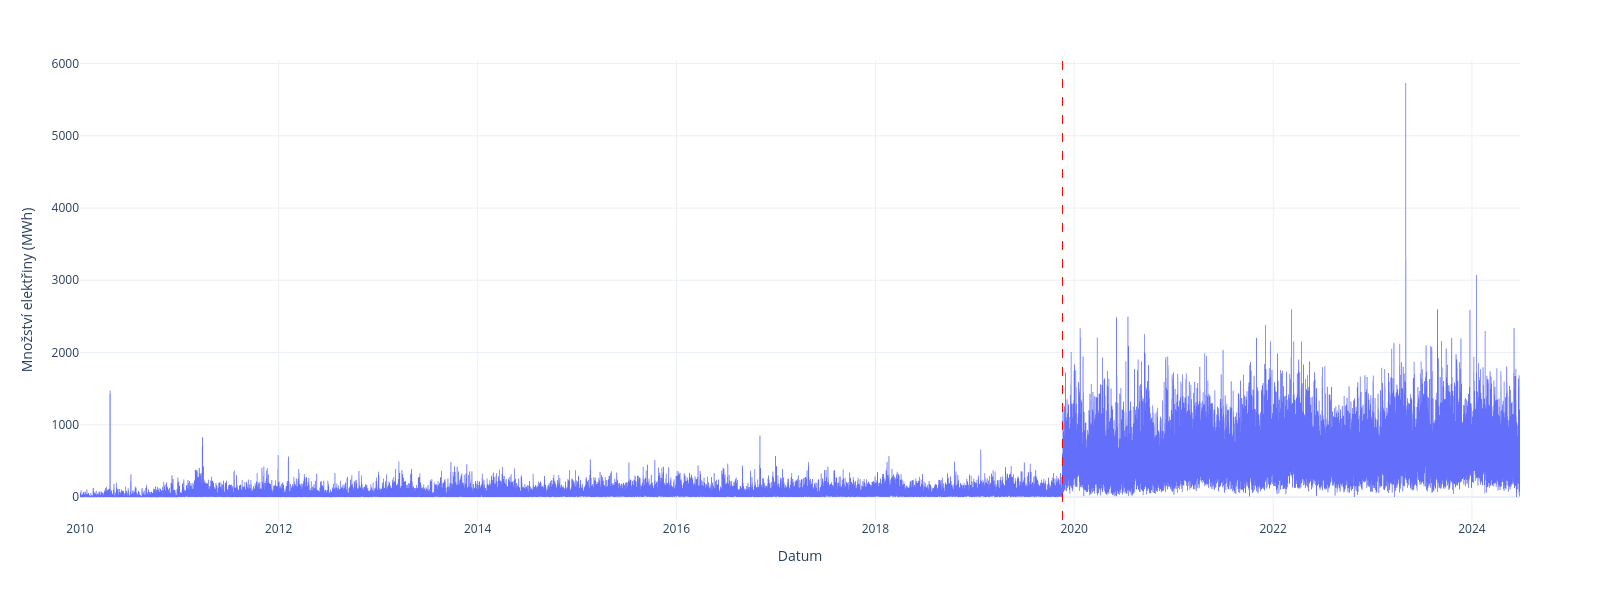
\includegraphics[width=\textwidth]{static/graphs/ote.png}
    \caption{Zobchodované množství elektřiny 2010--2024}
    \label{fig:ote}
\end{figure}

 
\subsubsection*{ČHMÚ} (Český hydrometeorologický ústav) musí zpřístupnit denní, měsiční a roční klimatologické charakteristiky za období 1961--2023. \footnote[2]{Zákon č. 123/1998 Sb., o právu na informace o životním prostředí.}

Denní úhrn doby trvání slunečního svitu je časový interval mezi východem a západem Slunce,
během kterého není sluneční kotouč zakrytý oblačností nebo jinými překážkami.
Fyzikálně je definován jako doba, kdy je intenzita toku přímého slunečního záření vyšší než 120 \si{\watt}/\si{\meter\squared}.
Udává se v hodinách.

% Na grafu \ref{fig:ote} je zobrazeno množství osvitových hodin od roku 2010 až po současnost.
% Z grafu je patrné, že v letních měsících je v průměru více osvitových hodin než v zimních.

% \href{https://www.chmi.cz/files/portal/docs/meteo/ok/open_data_2023/Podminky_uziti_udaju.pdf}{Podmínky užití dat}

\begin{figure}[H]
    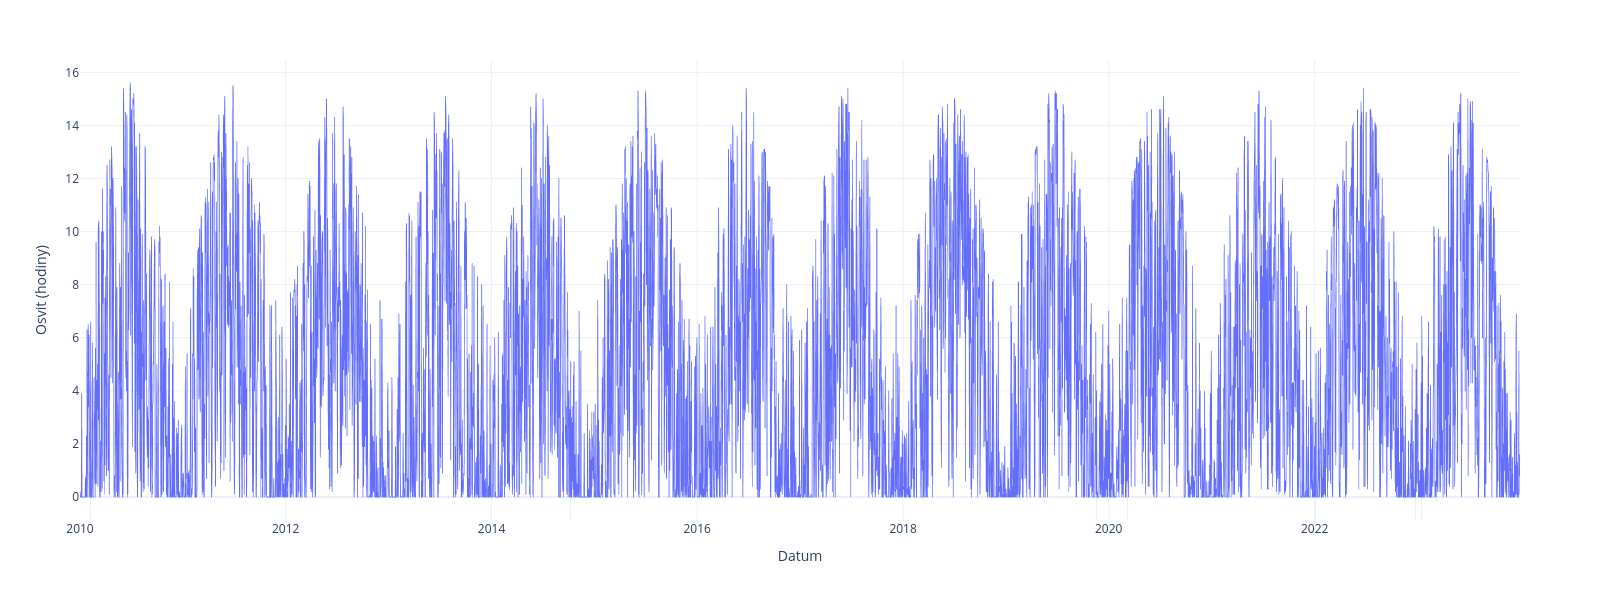
\includegraphics[width=\textwidth]{static/graphs/osvit.png}
    \caption{ČHMÚ. Osvitové hodiny 2010--2023}
    \label{fig:ote}
\end{figure}

\subsection{Optimalizační model}


\subsection{Metody API}

\subsubsection{Route 1} slouží k ...

\textbf{Metoda:} \texttt{GET}



\section{Konkrétní příklady}